% Created by tikzDevice version 0.12.5 on 2024-01-22 11:05:10
% !TEX encoding = UTF-8 Unicode
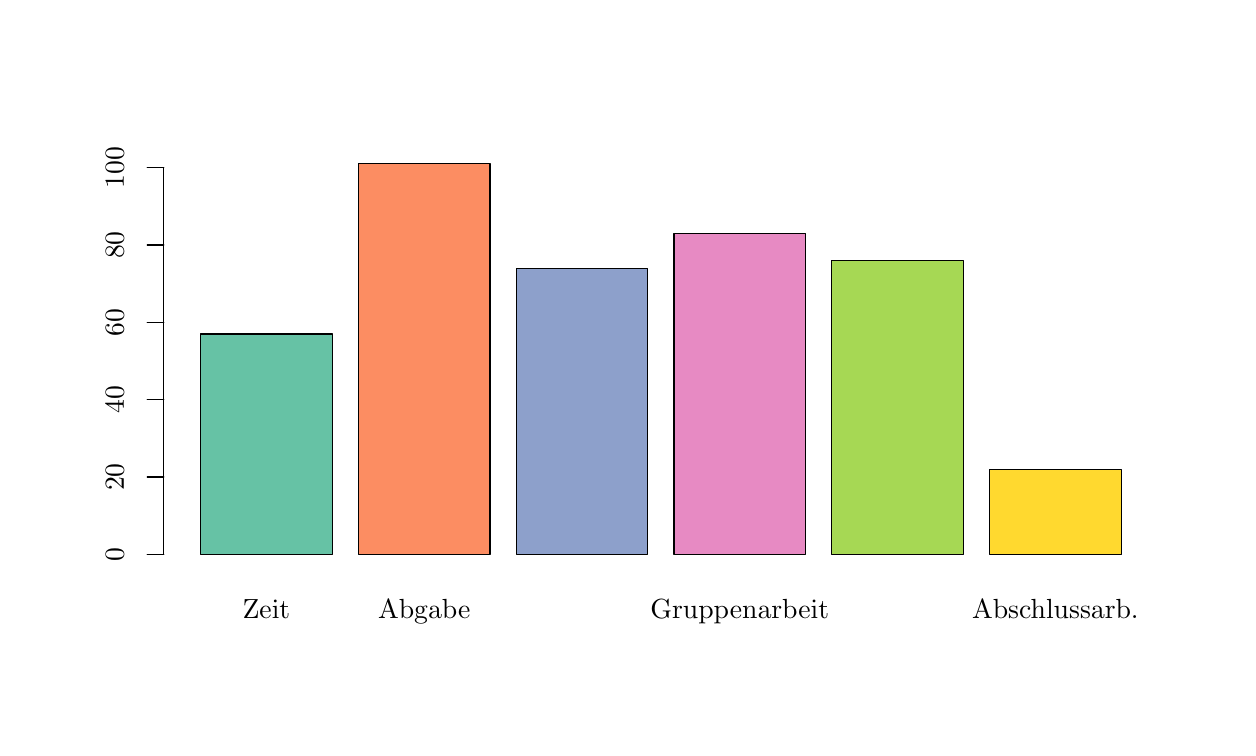
\begin{tikzpicture}[x=1pt,y=1pt]
\definecolor{fillColor}{RGB}{255,255,255}
\path[use as bounding box,fill=fillColor,fill opacity=0.00] (0,0) rectangle (433.62,252.94);
\begin{scope}
\path[clip] (  0.00,  0.00) rectangle (433.62,252.94);
\definecolor{drawColor}{RGB}{0,0,0}
\definecolor{fillColor}{RGB}{102,194,165}

\path[draw=drawColor,line width= 0.4pt,line join=round,line cap=round,fill=fillColor] ( 62.50, 62.61) rectangle (110.02,142.26);
\definecolor{fillColor}{RGB}{252,141,98}

\path[draw=drawColor,line width= 0.4pt,line join=round,line cap=round,fill=fillColor] (119.52, 62.61) rectangle (167.04,203.75);
\definecolor{fillColor}{RGB}{141,160,203}

\path[draw=drawColor,line width= 0.4pt,line join=round,line cap=round,fill=fillColor] (176.54, 62.61) rectangle (224.06,166.02);
\definecolor{fillColor}{RGB}{231,138,195}

\path[draw=drawColor,line width= 0.4pt,line join=round,line cap=round,fill=fillColor] (233.56, 62.61) rectangle (281.08,178.59);
\definecolor{fillColor}{RGB}{166,216,84}

\path[draw=drawColor,line width= 0.4pt,line join=round,line cap=round,fill=fillColor] (290.58, 62.61) rectangle (338.10,168.81);
\definecolor{fillColor}{RGB}{255,217,47}

\path[draw=drawColor,line width= 0.4pt,line join=round,line cap=round,fill=fillColor] (347.60, 62.61) rectangle (395.12, 93.35);
\end{scope}
\begin{scope}
\path[clip] (  0.00,  0.00) rectangle (433.62,252.94);
\definecolor{drawColor}{RGB}{0,0,0}

\node[text=drawColor,anchor=base,inner sep=0pt, outer sep=0pt, scale=  1.00] at ( 86.26, 39.60) {Zeit};

\node[text=drawColor,anchor=base,inner sep=0pt, outer sep=0pt, scale=  1.00] at (143.28, 39.60) {Abgabe};

\node[text=drawColor,anchor=base,inner sep=0pt, outer sep=0pt, scale=  1.00] at (257.32, 39.60) {Gruppenarbeit};

\node[text=drawColor,anchor=base,inner sep=0pt, outer sep=0pt, scale=  1.00] at (371.36, 39.60) {Abschlussarb.};

\path[draw=drawColor,line width= 0.4pt,line join=round,line cap=round] ( 49.20, 62.61) -- ( 49.20,202.35);

\path[draw=drawColor,line width= 0.4pt,line join=round,line cap=round] ( 49.20, 62.61) -- ( 43.20, 62.61);

\path[draw=drawColor,line width= 0.4pt,line join=round,line cap=round] ( 49.20, 90.56) -- ( 43.20, 90.56);

\path[draw=drawColor,line width= 0.4pt,line join=round,line cap=round] ( 49.20,118.51) -- ( 43.20,118.51);

\path[draw=drawColor,line width= 0.4pt,line join=round,line cap=round] ( 49.20,146.45) -- ( 43.20,146.45);

\path[draw=drawColor,line width= 0.4pt,line join=round,line cap=round] ( 49.20,174.40) -- ( 43.20,174.40);

\path[draw=drawColor,line width= 0.4pt,line join=round,line cap=round] ( 49.20,202.35) -- ( 43.20,202.35);

\node[text=drawColor,rotate= 90.00,anchor=base,inner sep=0pt, outer sep=0pt, scale=  1.00] at ( 34.80, 62.61) {0};

\node[text=drawColor,rotate= 90.00,anchor=base,inner sep=0pt, outer sep=0pt, scale=  1.00] at ( 34.80, 90.56) {20};

\node[text=drawColor,rotate= 90.00,anchor=base,inner sep=0pt, outer sep=0pt, scale=  1.00] at ( 34.80,118.51) {40};

\node[text=drawColor,rotate= 90.00,anchor=base,inner sep=0pt, outer sep=0pt, scale=  1.00] at ( 34.80,146.45) {60};

\node[text=drawColor,rotate= 90.00,anchor=base,inner sep=0pt, outer sep=0pt, scale=  1.00] at ( 34.80,174.40) {80};

\node[text=drawColor,rotate= 90.00,anchor=base,inner sep=0pt, outer sep=0pt, scale=  1.00] at ( 34.80,202.35) {100};
\end{scope}
\end{tikzpicture}
